%%%%%%%%%%%%%%%%%%%%%%%%%%%%%%%%%%%%%%%%%%%%%%%%%%%%%%%%%%%%%%%%%%%%%%%%%%
\chapter{Optimalizace velikosti bajtkódu}\label{Tool}

% TODO 
% *


%\section{?}
%\section{?}

%%%%%%%%%%%%%%%%%%%%%%%%%%%%%%%%%%%%%%%%%%%%%%%%%%%%%%%%%%%%%%%%%%%%%%%%%%
\section{Analýza bajtkódu}\label{Analysis}

% Popis způsobu analýzy rozsáhlého vzorku testovacích dat, prezentace výsledků a zhodnocení.

V~této kapitole popisuji výsledky analýzy bajtkódu. Pomocí nástroje \texttt{jbyco} jsem získala data reprezentující vybraný vzorek testovacích souborů a tato data následně zpracovala a vyhodnotila. Zkoumala jsem velikosti položek v~\texttt{class} souborech, využití lokálních proměnných a parametrů metod a typické sekvence instrukcí.

Testovací vzorek jsem vytvořila z~\texttt{jar} souborů stažených z~\texttt{http://mvnrepository.com}. Z~populárních kategorií jsem vybrala nejčastěji stahované soubory. Pracovala jsem se dvěmi testovacími vzorky. Velký vzorek se skládal z 95 souborů o celkové velikosti 102,4 MB a obsahoval 59 229 \texttt{class} souborů. Menší vzorek se skládal z 80 souborů o velikosti 46,6 MB a obsahoval 27 981
\texttt{class} souborů. Menší vzorek jsem použila pro vyhledání typických sekvencí instrukcí.

\subsubsection{Velikost položek v souboru}

Typický \texttt{class} soubor z velkého vzorku obsahuje v průměru 117 konstant v tabulce konstant, 2 členské proměnné, 8 metod, 163 instrukcí a 29 atributů. Ze zkoumání celkové velikosti těchto položek vyplynulo, že 64\% z celkové velikosti všech souborů tvoří konstanty, 0,7\% členské proměnné bez konstant, 2,1\% metody bez konstant a atributů a 10\% instrukce.

Při bližším pohledu na velikosti konstant se ukázalo, že 57\% z celkové velikosti souborů tvoří pouze konstanty typu \textit{constant\_utf8}. Tedy konstanty popisující řetězce. Velikosti ostatních konstant jsou zanedbatelné. Řetězce popisující názvy a typy tříd, metod a členských proměnných tvoří 61\% z celkové velikosti konstant typu \textit{constant\_utf8}.

Součet velikostí všech atributů ku celkové velikosti souborů tvoří 47\%, ale tato hodnota je nepřesná, neboť atributy mohou být součástí jiných atributů a jejich velikost je tedy započítána vícekrát. Nejvýznamnější z hlediska velikosti jsou atribut \texttt{Code} s velikostí 30\% z celkové velikosti souborů a součet velikostí informativních atributů s velikostí 14\%.

Zkoumání instrukcí z hlediska jejich velikosti ukázalo, že prvních pět nejobjemnějších instrukcí tvoří 40\% z celkové velikosti instrukcí. Jsou to instrukce pro volání metod, načtení hodnoty z členské proměnné a načtení reference na objekt z lokální proměnné s indexem 0. Na této pozici se často vyskytuje reference na aktuální objekt. Z instrukcí s proměnnou délkou má instrukce \texttt{tableswitch} v průměru velikost 107 B a instrukce \texttt{lookupswitch} velikost 43 B.

% TODO tabulka celkových velikostí
% TODO tabulka řetězců
% TODO tabulka informativních atributů
% TODO tabulka nejčastějších instrukcí

\subsubsection{Využití lokálních proměnných a parametrů metody}

Data popisující využití parametrů a lokálních proměnných jsou znázorněna v grafech \ref{params} a \ref{vars}. Z dat vyplývá, že z lokálních proměnných obsahujících argumenty metody se tyto hodnoty načtou průměrně jedenkrát a dále se s nimi nepracuje. S nižším indexem proměnné počet načítání roste až k hodnotě 2,544 pro index 0. V tomto indexu se u nestatických metod předává reference na aktuální objekt (\texttt{this}). S lokálními proměnnými, které neslouží k předávání parametrů, se průměrně provádí 4,18 operací načítání, 1,76 operací vkládání a 0,25 operací inkrementace.

\begin{figure}[h!]
\centering
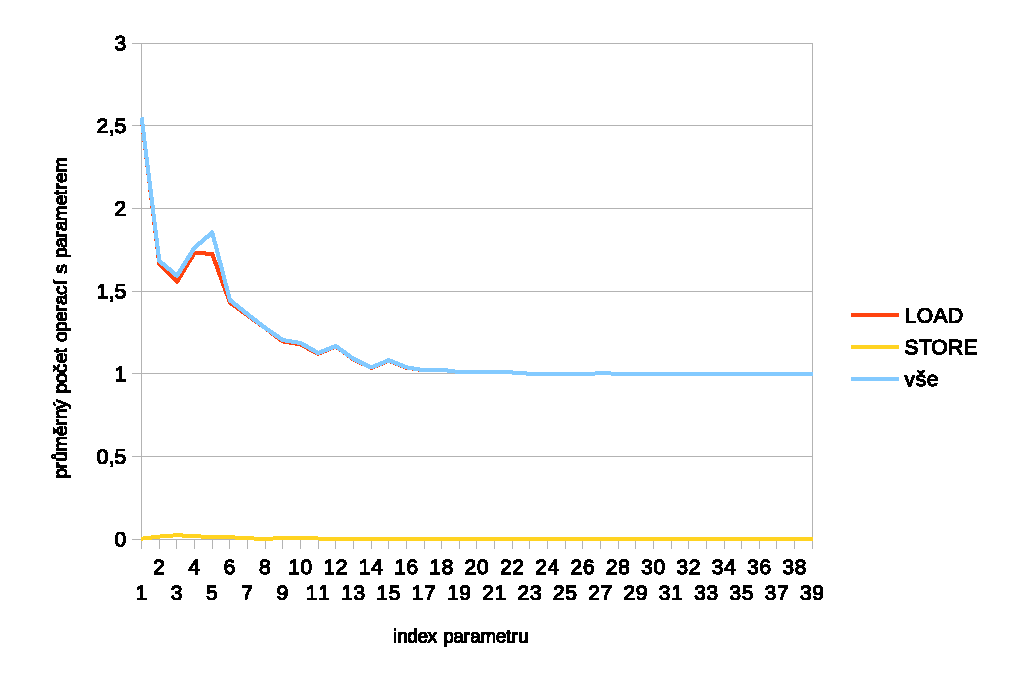
\includegraphics[scale=0.9]{fig/params}
\caption{Průměrné počty operací s parametry metod.}\label{params}
\end{figure}

\begin{figure}[h!]
\centering
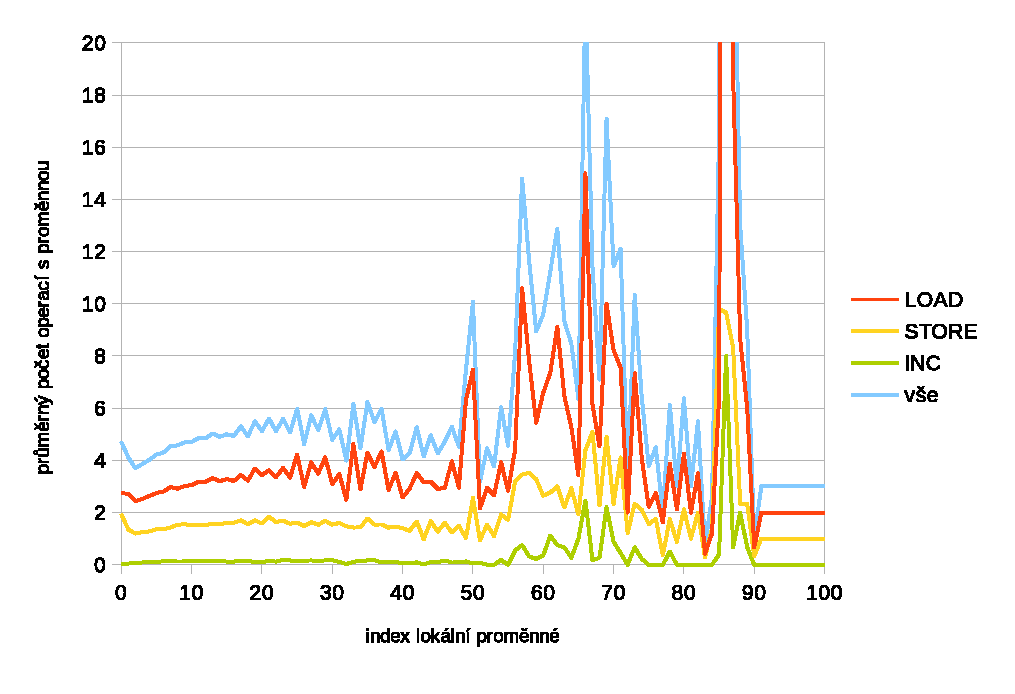
\includegraphics[scale=0.9]{fig/locals} 
\caption{Průměrné počty operací s lokálními proměnnými.}\label{vars}
\end{figure}

% TODO vzory
\subsubsection{Typické sekvence instrukcí}

Data pro zkoumání typických sekvencí instrukcí jsem získala pro různé kombinace parametrů popisujících úroveň abstrakce instrukce. Za maximální délku zkoumané sekvence jsem zvolila 10 u sekvencí bez divokých karet a 5 u sekvencí s divokými kartami. Práh pro prořezání stromu sekvencí dosáhl nejvyšší hodnoty 6. Taková hodnota je zanedbatelná a nemohla výrazně ovlivnit získaná data. 

% patterns_o1_p1_0_1.out, obsahuje další zajímavé případy swichů.

Z dat pro sekvence délky jedna vyplývá, že 15,80\% instrukcí tvoří instrukce pro volání metod objektu. Také instrukce pro práci s lokálními proměnnými tvoří velkou část všech instrukcí: instrukce pro načtení hodnoty z lokální proměnné 10,96\%, z parametru metody 5,10\% a instrukce pro načtení reference na aktuální objekt 9,06\%. Na druhou stranu instrukcí pro ukládání hodnot do lokálních proměnných je výrazně méně: instrukce pro uložení hodnoty do lokální proměnné 4,03\%, do parametru metody 0,22\% a v 49 případech byla hodnota uložena do reference na \texttt{this}. To poukazuje na příliš časté načítání hodnot, které se nemění. Obdobně instrukce pro získání hodnoty z členské proměnné tvoří 4,53\%, instrukce pro ukládání hodnoty 1,70\%. Pro statické členské proměnné je to 1,16\% a 0,30\%. Z instrukcí pro načtení konstantní hodnoty jsou nejčastějšími typy \texttt{int} 5,91\%, řetězec 2,46\%, reference na \texttt{null} 0,61\%, \texttt{double} 0,24\% a \texttt{long} 0,24\%. Nejčastější instrukcí skoku je nepodmíněný skok 1,77\%. Následují skoky s testy na rovnost 1,22\%, \texttt{null} 0,53\% a nerovnost 0,50\%. Z hlediska práce se zásobníkem jsou zajímavé instrukce pro duplikaci a odebrání vrcholu, které tvoří 3,53\% a 0,88\%. Pro práci s polem pak instrukce pro uložení hodnoty 1,69\%, načtení hodnoty 0,62\% a zjištění délky pole 0,27\%. Ukládání hodnot do pole je tedy častější operací než čtení hodnot z pole. U proměnných to bylo naopak. Kromě instrukce pro vytvoření nového objektu 1,96\% a instrukcí pro označení návěští je četnost každé další instrukce pod 1\%. Z těchto instrukcí stojí za zmínku instrukce \texttt{swap} 0,02\%, \texttt{nop} 364 výskytů a instrukce \texttt{lookupswitch} a \texttt{tableswitch}. Ve 21 případech instrukce \texttt{lookupswitch} obsahovala jen adresu výchozího bloku instrukcí, v 552 případech obsahovala jednu dvojici hodnota-adresa a v 998 případech dvě dvojice, což je nejčastější podoba této instrukce. V instrukci \texttt{tableswitch} se nejčastěji pracuje s rozsahem hodnot o délce tři a to ve 442 případech. Ve 150 případech je délka rozsahu 1.

% patterns_o2_p1_0_1.out, patterns_o1_p3_0_1.out - lze zjistit typické hodnoty swichů

Při pohledu na konkrétní typy instrukcí je nejčetnější instrukcí \texttt{ALOAD this} s četností 9,06\%. Z instrukcí pro návrat z metody jsou typickými instrukce \texttt{areturn} 2,13\%, \texttt{return} 1,68\% a \texttt{ireturn} 0,85\%. Nejčastěji se pracuje s proměnnými a poli typu reference na objekt a \texttt{int}. Ze zkoumání konkrétních parametrů instrukcí vyplývá, že nejčastějšími konstantními hodnotami typu \texttt{int} jsou 0, 1, 2, 3, 4, -1, 8, 5, 10, 7, 16 a 255. Typickou konstantou typů \texttt{long} a \texttt{double} je 0 a typickou řetězcovou konstantou je prázdný řetězec. Nejčastější třídou, se kterou se v instrukcích pracuje, je \texttt{java.lang.StringBuilder}. Další typické třídy jsou \texttt{java.lang.Object} a \texttt{java.util.Iterator}.

% patterns_o1_p1_0_2.out

Nejvyskytovanější se dvojicí instrukcí je sekvence pro načtení hodnoty členské proměnné aktuálního objektu. Dalšími dvojicemi jsou: duplikace reference na právě vytvořený objekt, načtení hodnot ze dvou proměnných, uložení návratové hodnoty metody do proměnné, uložení hodnoty do nějaké proměnné následované vložení hodnoty z nějaké proměnné, volání metody, kde parametrem je řetězcová konstanta, volání metody s hodnotou členské proměnné jako parametrem, zahození návratové hodnoty volané metody, volání metody, kde parametrem je celočíselná hodnota typu \texttt{int}, kontrola typu objektu vráceného metodou, načtení hodnoty členské proměnné do lokální proměnné a vložení celočíselné hodnoty do pole nebo proměnné. Četnost ostatních dvojic je méně než 0,09\%. Ze dat dále plyne, že z celkového počtu 504 741 zkoumaných metod jich 39 317 mělo prázdný seznam instrukcí. První instrukcí v seznamu instrukcí je typicky instrukce \texttt{load this}. 

% patterns_o1_p1_0_3/4.out - delší sekvence nejsou v tomto případě už zajímavé

Z typických trojic instrukcí je zajímavá sekvence, která uloží na index pole daný celočíselnou konstantou konstantní hodnotu typu \texttt{int}. Sekvence se nejspíše používá k inicializaci pole. Méně častou operací je přiřazení hodnoty z lokální proměnné na konstantní index pole. 

% patterns_o1_p2_0_10.out
Z toho soubory mne zajímaly pouze sekvence s opakujícími se parametry. Dvojice instrukcí, které uloží hodnotu do proměnné a tutéž hodnotu načtou zpět z téže proměnné na zásobník, má relativní četnost 0,12\%. Přitom hodnota proměnné se nemůže změnit. Vhodnější by proto bylo hodnotu duplikovat a kopii vložit do proměnné. Obdobně dochází k opakovanému vkládání téže celočíselné konstanty (0,01\%), opakovanému načítání hodnoty z téže lokální proměnné (0,002\%). Opakovaná kontrola instrukcí \texttt{checkcast}, zda je objekt daného typu, je také zbytečná. K nepodmíněnému skoku na bezprostředně následující instrukci dochází ve 841 případech. Takovou instrukci lze vynechat. Další zbytečnou operací je opakované vkládání řetězcové konstanty (718 případů). V sekvencích instrukcí, kde je hodnota uložena do proměnné, načtena zpět z téže proměnné a následně použita jako návratová hodnota funkce, případně zahozena, je práce s lokální proměnnou zbytečná a instrukce lze vynechat.




% Zkoumání krátkých těl metod

% Zkoumání duplicitních operací

% Zkoumání switch

% Hledání cyklů


%%%%%%%%%%%%%%%%%%%%%%%%%%%%%%%%%%%%%%%%%%%%%%%%%%%%%%%%%%%%%%%%%%%%%%%%%%
\section{Metody pro optimalizaci velikosti bajtkódu}\label{Analysis}


%=========================================================================

